\chapter{Implementation}
\label{chap:Impl}
\section{Programming APIs}

To implement VR applications, we can work directly with the SDK provided from each headset manufacturer, the advantage is that we can interact at a low level with the devices.\\ 
Another way is to use an SDK of a well-defined standard for example OpenVR from Valve or OpenXR from the Khronos group. This allows us to write applications for a target group of devices like 6-DOF supporting headsets without having to deal with different manufacturer SDKs (see Figure \ref{fig:openxr-overview}). On a side note: the X in OpenXR means that the specification is not only used for virtual reality (VR) applications but also for augmented reality (AR) and other technologies (XR) possibly proposed in the future.\\
Lastly, we can work with different engines which will provide with additional features. While classical desktop engines rely on downloading a complete bundled software package for distributing the application, WebXR and WebVR allow us to distribute and run our application via the browser, similar to WebGL.

At the time of writing, the OpenXR and WebXR specification is still relatively new being in its first revision therefore it is not implemented by each headset manufacturer, browser and engine yet. However, these standards are meant to replace the old OpenVR and WebVR in the future.

\begin{figure}[h]
    \centering
    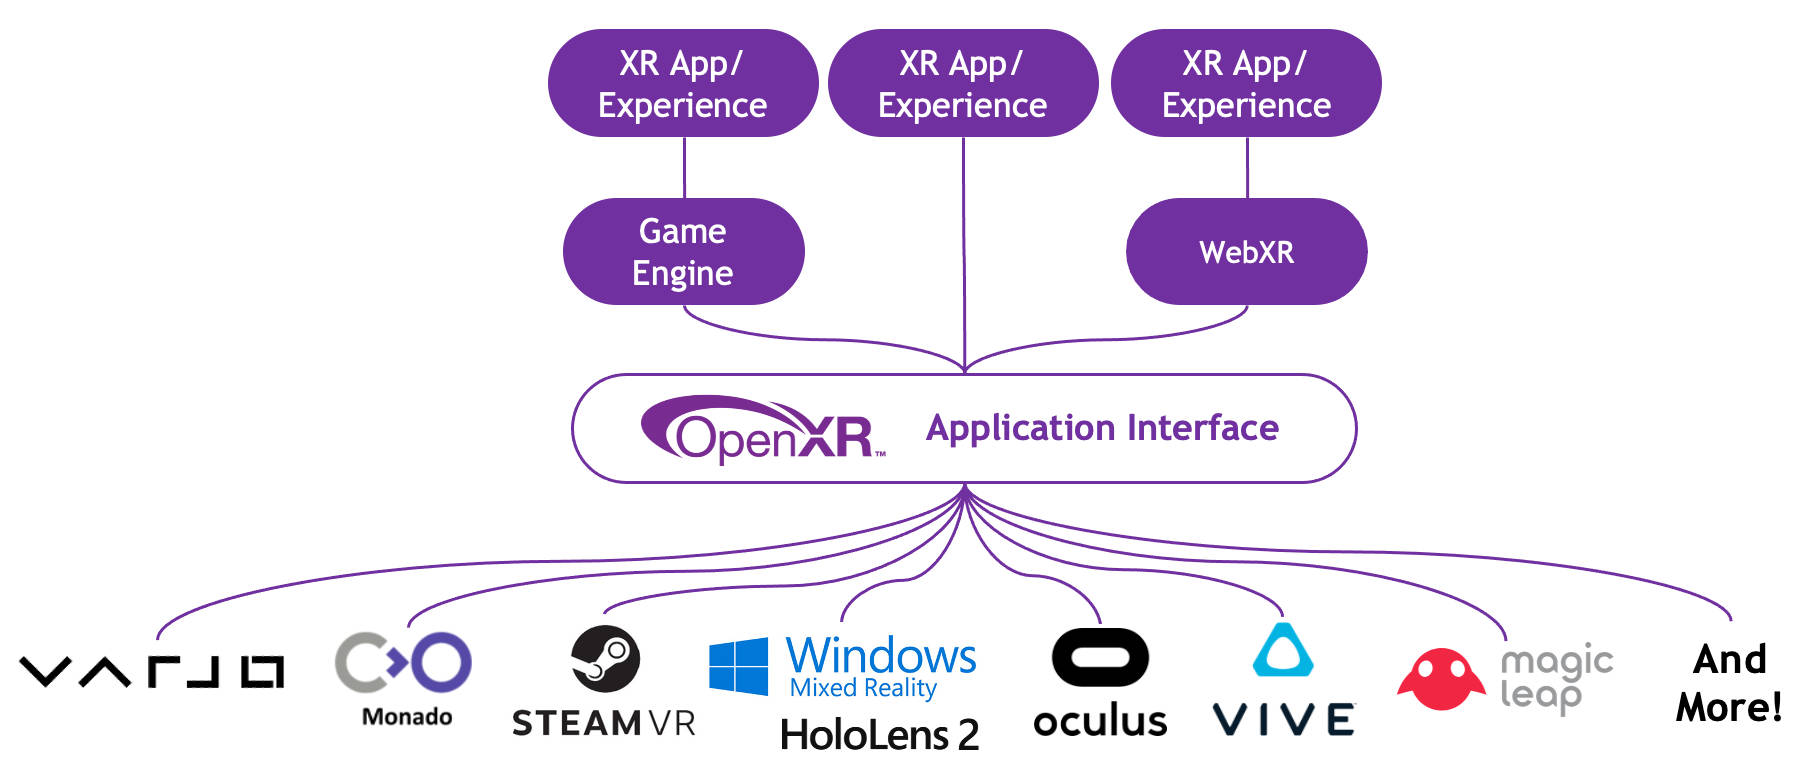
\includegraphics[width=\textwidth]{graphics/openXR-overview.jpg}
    \caption{Overview of the OpenXR API Stack \cite{khronosGroupOpenXR}}
    \label{fig:openxr-overview}
\end{figure}

\section{Prior Publication}

\section{Technology}

\section{Program Overview}

\subsection{Data Structure}

\subsection{Program Flow}
\begin{figure}[h]
    \centering
    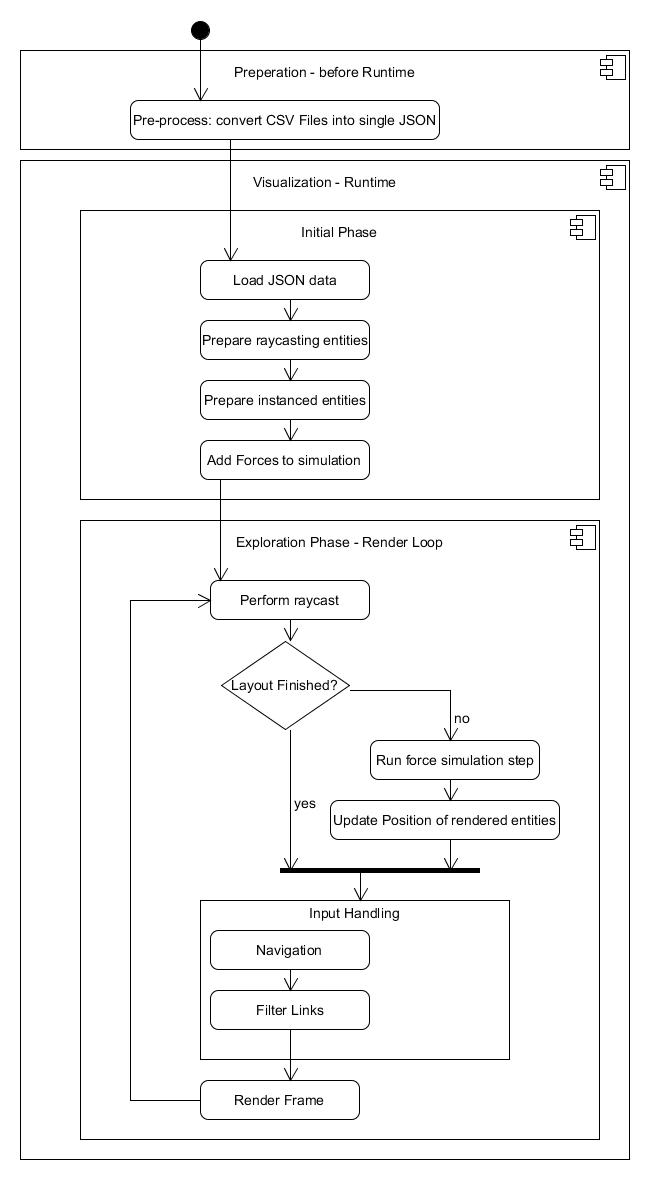
\includegraphics[width=0.74\textwidth]{graphics/vrgraph_flow.jpg}
    \caption{Program flow of our Implementation.}
    \label{fig:impl_programFlow}
\end{figure}

\subsection{Virtual Scene Graph}
2 Virtual Object Arrays
Raycasting Objects
Rendered Objects

\section{Program Details}

\subsection{Preprocessing Scripts}

Flexible transforming any CSV Data to our own data format \\
generation of test data \\
coloring, filtering, ... parameter \\
File Format of final processed .JSON for the actual web-based visualization \\

\subsection{Layout calculation}
Implementation Details of Forces, \\
Optimization for Saving Pos and set after done

\subsection{Rendering}
Goal of Rendering: 
Performance, Support Transparency of nodes. 

Instancing per Links, 
Instancing per Hierarchical Layer of nodes, 
Transparency,
Wireframe

\subsection{VR Interactions}
Camera Rig vs Camera
camera rotation, correct position 
\\
extend controller
\\
Teleport
\\
FreeFly

\subsection{Scale}
Move + Scale\\
Animation
\\

\subsection{Filtering}
Filtering of Links\\
Algorithmus multilayer detail layout\\
